%root=main.tex
\section{System Model}
\label{sec_basic_model}

We build the basic model of a charging station,
and analyze whether or not Tesla can support a successful migration to all-electric personal transpotations in the United States from the energy perspective.

\subsection{The Standard of Feasibility}
\label{subsec_standard_feasibility}
In order to evaluate the feasibility of supporting a successful migration to all-electric personal transpotations in the United States,
we firstly need to define feasibility.
\begin{definition}
\textbf{Solution Feasibility:}
\label{def_feasibility}
Suppose $Solution(a)$ is the solution of the target area $a$,
the solution of charging stations is feasible if and only if:
(1) it can meet the \textbf{charging demand} in target area $a$,
(2) it can let the vehicle get to anywhere (\textbf{coverage}) in target area $a$.
\end{definition}
In Definition~\ref{def_feasibility}, coverage can be regarded as the Connectivity of the networking graph in area $a$ mentioned in Section~\ref{sec_profile_us},
but it is hard to quantify the charging demand in area $a$.
To solve this issue,
we refer to the previous work about the layout of electric vehicle charging station~\cite{wang2010novel},
Note that it is reasonable to quantify the charging demand from the energy perspective.
Here is the definition of the charging demand.
\begin{definition}
\textbf{Charging Demand:}
\label{def_charging_demand}
Suppose $Demand(a)$ is the charging demand of the target area $a$,
$R_{electic}(a)$ is the penetration rate of electric vehicles in target area $a$,
and $E_{consume}(a)$ is the energy consumed by traffic of $a$,
then we have the equation:
\begin{equation}
\label{equ_demand}
Demand(a) = E_{consume}(a) \times R_{electric}(a)
\end{equation}
\end{definition}
Suppose the set of the charging stations in $a$ is $Set(a)$,
$Set_i(a)$ represents a specific charging station $i$ and the energy it can provide is $E(Set_i(a))$.
If and only if the solution can meet the equation:
\begin{equation}
\label{equ_energy}
\sum{E(Set_i(a))} (i \in Set(a)) \geqslant Demand(a)
\end{equation}
Then, we say the solution can meet the charging demand of target area $a$.

For the distribution of charging demand in target area $a$,
without considering its shape, we suppose the leaving vehicles and the entering vehicles are equal in quantity,
then the number of the vehicles in area $a$ should be a constant, denoted as $N_{a}$.
This factor should depends on \textbf{population density} and \textbf{wealth condition}(the electric vehicle penetration rate $R_{electic}(a)$) of $a$.

%\subsection{The Model of Charger Station}


%We suppose the size of coverage area that a specific charging station can provide is circle.
%Thus, we can calculate the coverage area sizes of destination charging and supercharging respectively:


\subsection{The Model of City}
For the model of the city,
we treat a city $a$ as an undirected graph $G_{a}(Po(a),\theta(a))$.
This idea has been proved to be reasonable by the work~\cite{lam2014electric}.
Specifically, $Po(a)$ denotes the set of possible sites for constructing charging station,
and $\theta(a)$ denotes the set of roads connecting pairs of sites.
Let $d(i, j)$ denotes the distance of the shortest path from $i$ to $j$ by traversing the roads in $\theta(a)$,
which can be calculated by Dijkstra's Algorithm~\cite{Dijkstra}.
Note that, here $d(i, j)$ refers to the distance of an actual road connecting sites $i$ and $j$ but not the Euclidean distance.

Each site $i$ has a charging demand requirement $Demand(i)$ which is defined in Definition~\ref{def_charging_demand}
(\eg, the more electric vehicles in the coverage of the charging station located in $i$, the higher $Demand(i)$ is).
Let $Cap(i)$ be the capacity of node $i$ which represents the average capacity of charging service supported if a charging station is constructed at location $i$.

Considering the City model above, we can give the definition of the reachability.
\begin{definition}
\label{def_reachability}
\textbf{Reachability:}
Suppose $G_{a}(Po(a),\theta(a))$ is the graph of area $a$,
$Po(a)^{'}$ is the subset of $Po(a)$,
then we say anywhere in $Po(a)^{'}$ is reachable if and only if it can follow three conditions below:
\begin{condition}
\label{con_reach_1}
$\forall i \in Po(a)^{'} \Rightarrow \exists j \in Po(a)^{'},  d(i, j) \leqslant R$
\end{condition}
\begin{condition}
\label{con_reach_2}
$\forall i \in Po(a), Cap(i) = \sum{Cap(j)}, (j \in Po(a)^{i}, d(i, j) \leqslant \alpha{R}) \Rightarrow Cap(i) \geqslant Demand(i)$
\end{condition}
\begin{condition}
\label{con_reach_3}
$\forall i, j \in Po(a)^{i} \Rightarrow d(i, j)  \leqslant n_{ij}R, (n_{ij} \geqslant 1)$
\end{condition}
(Note that $\alpha \in (0,1]$ is the factor to describe the habit of recharging of drivers,
 $n_(ij)$ represents the amount of charging stations along the path $d(i, j)$)
\end{definition}

Condition~\ref{con_reach_1} means that any charging station in a specific location can recharge at another site within the range $R$,
which guarantees that any electric vehicle would not be restricted in one area.

Condition~\ref{con_reach_2} means that the local charging demand at a area must be satisfied by the total charging capacities contributed by those charging stations located within distance $\alpha{R}$ away.
Here, we use the factor $\alpha$ represents the habit of recharging of drivers.
(\eg, $\alpha = 0.75$ means that the driver would recharge the vehicle when the vehicle has consumed $75\%$ of the total energy.)

Condition~\ref{con_reach_3} says, in the charging station network, the vehicle can go by more than one charging stations to travel to another charging station.

In order to explain our model more clearly,
Figure~\ref{fig_city_model} shows a simple example of our model based on Los Angeles~\cite{LAMap}.


\begin{figure}[!t]
\centering
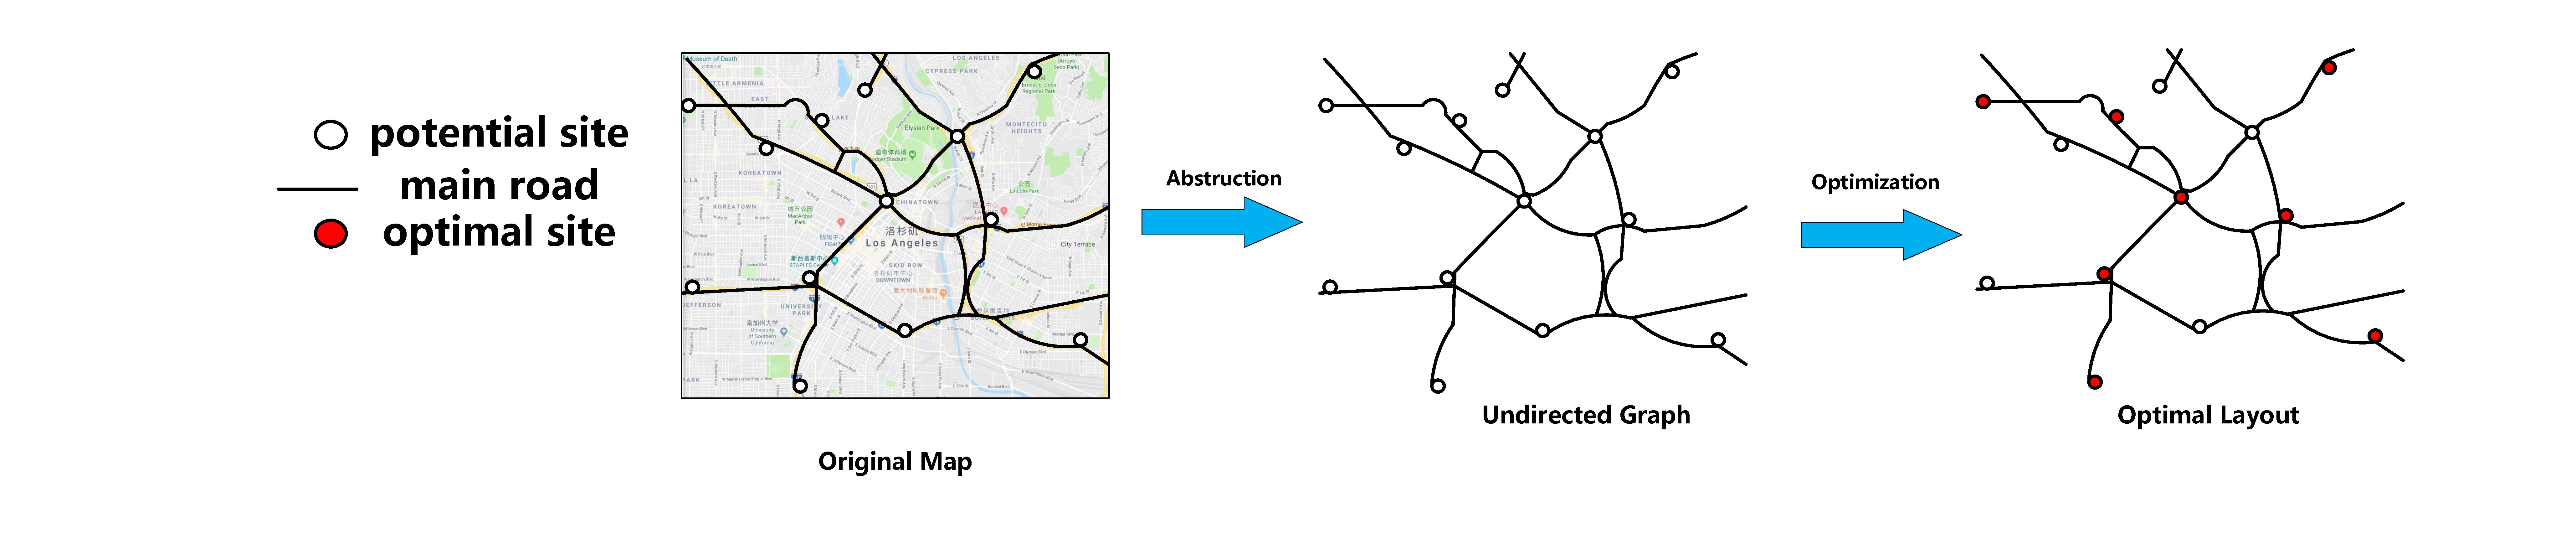
\includegraphics[width=6.7in]{city_model.pdf}
%\vspace{-0.1in}
\caption{An Example of our City Model.}
\label{fig_city_model}
%\vspace{-0.2in}
\end{figure}

